% This is "sig-alternate.tex" V2.0 May 2012
% This file should be compiled with V2.5 of "sig-alternate.cls" May 2012
%
% This example file demonstrates the use of the 'sig-alternate.cls'
% V2.5 LaTeX2e document class file. It is for those submitting
% articles to ACM Conference Proceedings WHO DO NOT WISH TO
% STRICTLY ADHERE TO THE SIGS (PUBS-BOARD-ENDORSED) STYLE.
% The 'sig-alternate.cls' file will produce a similar-looking,
% albeit, 'tighter' paper resulting in, invariably, fewer pages.
%
% ----------------------------------------------------------------------------------------------------------------
% This .tex file (and associated .cls V2.5) produces:
%       1) The Permission Statement
%       2) The Conference (location) Info information
%       3) The Copyright Line with ACM data
%       4) NO page numbers
%
% as against the acm_proc_article-sp.cls file which
% DOES NOT produce 1) thru' 3) above.
%
% Using 'sig-alternate.cls' you have control, however, from within
% the source .tex file, over both the CopyrightYear
% (defaulted to 200X) and the ACM Copyright Data
% (defaulted to X-XXXXX-XX-X/XX/XX).
% e.g.
% \CopyrightYear{2007} will cause 2007 to appear in the copyright line.
% \crdata{0-12345-67-8/90/12} will cause 0-12345-67-8/90/12 to appear in the copyright line.
%
% ---------------------------------------------------------------------------------------------------------------
% This .tex source is an example which *does* use
% the .bib file (from which the .bbl file % is produced).
% REMEMBER HOWEVER: After having produced the .bbl file,
% and prior to final submission, you *NEED* to 'insert'
% your .bbl file into your source .tex file so as to provide
% ONE 'self-contained' source file.
%
% ================= IF YOU HAVE QUESTIONS =======================
% Questions regarding the SIGS styles, SIGS policies and
% procedures, Conferences etc. should be sent to
% Adrienne Griscti (griscti@acm.org)
%
% Technical questions _only_ to
% Gerald Murray (murray@hq.acm.org)
% ===============================================================
%
% For tracking purposes - this is V2.0 - May 2012

\documentclass{sig-alternate}
\usepackage{graphicx}
\graphicspath{{images/}}

\begin{document}
%
% --- Author Metadata here ---
\conferenceinfo{WOODSTOCK}{'97 El Paso, Texas USA}
%\CopyrightYear{2007} % Allows default copyright year (20XX) to be over-ridden - IF NEED BE.
%\crdata{0-12345-67-8/90/01}  % Allows default copyright data (0-89791-88-6/97/05) to be over-ridden - IF NEED BE.
% --- End of Author Metadata ---

\title{{\ttlit Internet Outages} : Analysis of the Outages Mailing List}
%\titlenote{(Produces the permission block, and
%copyright information). For use with
%SIG-ALTERNATE.CLS. Supported by ACM.}}
%\subtitle{[Extended Abstract]
%\titlenote{A full version of this paper is available as
%\textit{Author's Guide to Preparing ACM SIG Proceedings Using
%\LaTeX$2_\epsilon$\ and BibTeX} at
%\texttt{www.acm.org/eaddress.htm}}}
%
% You need the command \numberofauthors to handle the 'placement
% and alignment' of the authors beneath the title.
%
% For aesthetic reasons, we recommend 'three authors at a time'
% i.e. three 'name/affiliation blocks' be placed beneath the title.
%
% NOTE: You are NOT restricted in how many 'rows' of
% "name/affiliations" may appear. We just ask that you restrict
% the number of 'columns' to three.
%
% Because of the available 'opening page real-estate'
% we ask you to refrain from putting more than six authors
% (two rows with three columns) beneath the article title.
% More than six makes the first-page appear very cluttered indeed.
%
% Use the \alignauthor commands to handle the names
% and affiliations for an 'aesthetic maximum' of six authors.
% Add names, affiliations, addresses for
% the seventh etc. author(s) as the argument for the
% \additionalauthors command.
% These 'additional authors' will be output/set for you
% without further effort on your part as the last section in
% the body of your article BEFORE References or any Appendices.

\numberofauthors{8} %  in this sample file, there are a *total*
% of EIGHT authors. SIX appear on the 'first-page' (for formatting
% reasons) and the remaining two appear in the \additionalauthors section.
%
\author{
% You can go ahead and credit any number of authors here,
% e.g. one 'row of three' or two rows (consisting of one row of three
% and a second row of one, two or three).
%
% The command \alignauthor (no curly braces needed) should
% precede each author name, affiliation/snail-mail address and
% e-mail address. Additionally, tag each line of
% affiliation/address with \affaddr, and tag the
% e-mail address with \email.
%
% 1st. author
\alignauthor
Guanyu Zhu
\email{zhuguanyu2010@gmail.com}
\alignauthor
Wei-Ting Lin
\email{wei-ting.lin@stonybrook.edu}
\alignauthor
Zhaowei Sun
\email{zhaowei.sun@stonybrook.edu}
       %
       %
       %
}
% There's nothing stopping you putting the seventh, eighth, etc.
% author on the opening page (as the 'third row') but we ask,
% for aesthetic reasons that you place these 'additional authors'
% in the \additional authors block, viz.
%\additionalauthors{Additional authors: John Smith (The Th{\o}rv{\"a}ld Group,
%email: {\texttt{jsmith@affiliation.org}}) and Julius P.~Kumquat
%(The Kumquat Consortium, email: {\texttt{jpkumquat@consortium.net}}).}
%\date{30 July 1999}
% Just remember to make sure that the TOTAL number of authors
% is the number that will appear on the first page PLUS the
% number that will appear in the \additionalauthors section.

\maketitle
\begin{abstract}
Internet outages are an essential topic for the contemporary society because of the popularity of mobile devices rises, and the broad scope existence of Internet services. A sudden Internet outages could cause several consequences such as companies are unable to work[1], students are unable to do their assignments[2] and even the finance of a country could drop down. If there is a way which can help us to analyze and predict the causes of Internet outages, Internet providers and the technicians will be able to solve the problems and repair the hardware more efficiently. Unfortunately, although people have already noticed how critical it is, the study of Internet outages is being obstructed by many reasons such as the benefits of the Internet providers, private information, and the inadequate open resources. One related paper[3] puts great effort on the Internet outage this topic, the authors use Natural Language Processing (NLP) and Machine Learning technique to analyze and categorize the keywords in the outage mailing list [4] in order to classify the cause and effect of the Internet outages.
\end{abstract}

\section{Datasets}
\paragraph{In this section, we introduce the basic idea about the data that we use in this project such as where the data is obtained, what the data is use for, what the data looks like and how do we use the data for our project}
~\\
The outages mailing list (the data)[7] reports outages related to failures of major communications infrastructure components. It intends to share information so that network operators and end users can assess and respond to major outages. The list contains outage reports as well as post-mortem analysis and discussions on troubleshooting. 						
\par We download and analyze the outages mailing list taken on March, 2015 containing threads since its inception in 2006 [7]. It contains nine years discussions on the mailing list. These discussions are organized into thousands of  threads. Each thread contains a host-post, and it might also contain several replies. However, no matter a host-post or a reply, each of them contains poster’s information, subject, message, system information and a unique message ID. In our implementation, the usage of this data is to extract the subject and the contain of each host-post or reply and to assign each contain with the same subject to the same thread. In Figure 1, we show the first email, last email, total amount of posts, replies and threads.

\begin{figure}[h]
\centering
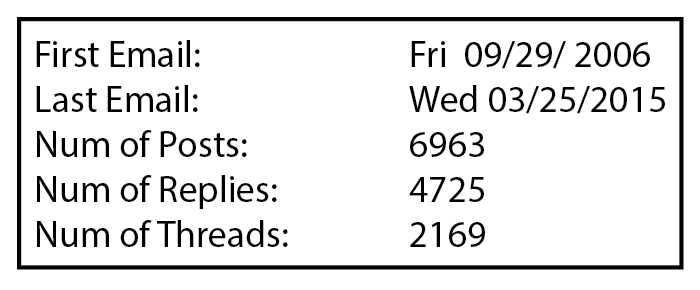
\epsfig{file=222.eps, height=1.1in, width=2.5in}
\caption{Datasets}
\end{figure}

\par Apparently, the number of replies is always lower than the number of posts. The reason why the number of threads is lower than the number of post is because two individual post might involve in the same subject. We consider them as the same thread in our implementation. Even though the number of posts in each month changes dramatically, Figure 2 shows that the average number of threads do not change dramatically in each month. For the midterm report, we use about 30 threads to be our test data and implement our classifier. 

\begin{figure}[h]
\centering
\epsfig{file=2.eps, height=1.5in, width=3in}
\caption{Num of Posts and Threads in the datasets}
\end{figure}

\section{Maillist text analysis}
\paragraph{In this section, we discuss how we extract keywords from the e-mail postings and present preliminary analysis of topics over time}
~\\
\textbf{Data Processing} 
\par The fact that maillist threads are comprised of natural language text which means that they are rich with semantic information underlying the failure, but also presents a challenge in terms of automatically parsing and processing the data. To address this challenge we employ techniques from text mining and natural language processing (NLP).

\subsection{Merge the posts that belongs to the same threads}
In general, we consider the dataset at the level of threads. Each thread consists of the set of e-mail messages (posts) in the thread. For each thread we extract relevant information ex. term and phrases.
After removing quoted text (text from previous emails in the thread included in each email) from its posts, we remove the content which is unimportant and fixed repeating such as the content between \textit{“BEGIN PGP SIGNATURE”} and \textit{“END PGP SIGNATURE”}, empty lines, poster information (ex: name) and post information (ex: date) that are not helpful for our final classifier.
\par Because the format of the original files is sometimes out of order; hence, we write a program fix.py and use it to  run through all the files and adjust the order of the content so that we can process the files and remove the system’s repeating content by our fliter.py easily.. Eventually, we save all different subjects of threads, assign contents of original posts and reply posts to each thread by using their Subjects and References and generate the processed files.

\subsection{Remove unrelated content of the thread}
In this part, we remove the unrelated content in every subject and thread. What is the meaning of unrelated content ? Those are some kinds of words those are useless for analyzing the network outage. We classify those unrelated contents into 9 categories

\begin{enumerate}
  \item Spurious data. We firstly remove those spurious data, which contained the identifying e-mail signatures used by posters and some data added by system or antivirus software. For example, “This message has been scanned for viruses and dangerous content by MailScanner, and is believed to be clean.” We treated this kind of message as the spurious data and should be discarded. 
  \item Links. Then we ignored the url, website links and email links in the posts. Those are has little things with the outage of network.
  \item Punctuations and Numbers.
  \item Traceroute measurements. We think these info are useless because only based on the traceroute measurements we can figure out the root cause of an incident.
  \item Stop words(e.g., articles, prepositions and pronouns). We also use a list of stop words obtained from the SMART information retrieval system[5].
  \item Organization and Human names. These organization and Human names are no meaning for us to analyze the cause of outage, such as Sprint, AT\&T, Gary, Tim, etc.
  \item Time-related and Place-related words. Such as day, night, NYC, San Jose, etc.
  \item Some unrelated abbreviation words. Such like ICS, ISP, etc.
  \item Others.  This includes some entities words( like issue,information, etc) or phrase(like “in order to”) that have nothing with network but can affect the efficiency and accuracy about the NLP(natural language processing) analysis.\ldots
\end{enumerate}
Compared with the methods mentioned in the reference paper[3](which only removes about 4 above kinds of words), we can make our NLP analysis be more accurate and efficient.

\subsection{Stemming and Lemmatization}
After step 2, the remaining words should be stemmed and  lemmatized (the process of grouping together the different inflected forms of a word) using python Natural Language Toolkit(NLTK) so they can be analyzed as a single item. For example, determining that “walk”, “walked” and “walking” are all forms of the same verb: “to walk”. Note that the simple stemming (i.e., walking to walk) does not suffice as it cannot differentiate the parts of speech based on context: e.g., when the term “meeting” acts as a verb: “we are meeting tomorrow” vs. a noun “let’s go to the meeting”. 
\par Lemmatization, on the other hand, can identify these contextual differences. The reason for doing stemming and Lemmatization is to decrease the dimension of the data, because “person” and “persons” have the same effect and meaning in the data for classifying the outage type, if we regard them as different word, it does not improve the classification effect but increase the dimension of the data, it will decrease the efficiency of running time and even the accuracy of our classification.

\subsection{TF-IDF}
After the step 3, at first, our initial idea is to use TF-IDF algorithm[6] of python Natural Language Toolkit (NLTK) to filter out words with tf-idf values less than 0.2. Low tf-idf value indicates that the word is very common throughout the dataset, and it is not useful for the data to use the classification method to classify the type of outage. But after we use TF-IDF algorithm to get the high value words, we found that some high tf-idf value words also have no effect for our outage type classification. 
\par From the Table 1 we can see that the word “david” has a high tf-idf value in the thread that we choose, but this word is a “name of person” word that has no any influence for our network outage type classification. If we use this word just because its high tf-idf value, it will increase the noise of our data and may influence the accuracy of our classification. Hence, we import the name-word library and city-word library of python Natural Language Toolkit(NLTK) to the unrelated content of thread.

\begin{table}
\centering
\begin{tabular}{ | l || c | }
  \hline
  david & 2.04769284337  \\
  \hline
  everydns & 1.82454929205  \\
  \hline
  ulevitch & 1.37042001196  \\
  \hline
  personal & 1.37042001196  \\
  \hline
  explanation & 1.37042001196  \\
  \hline
  net & 1.23676262715  \\
  \hline
\end{tabular}
\caption{TF-IDF Value}\label{table:tf-idf}
\end{table}

\subsection{Generate 2-dimension matrix for classification}
After step 4 we recompute the term frequency in the dataset and generate the 2-dimension matrix for term frequency. Every row indicates the different thread, every column indicates the different word that appears in the dataset. Once we get the matrix, we can use this matrix to do the classification because this is the “true” data that we want.

\section{Classification Methodology}
\paragraph{The terms and phrases extracted in our initial processing give a high-level view of the discussions on the mailing list. In this section, we discuss a classification methodology to help us systematically categorize the outages over time}

\subsection{Labeling}
First, based on the network knowledge base and general network outage types, we classify outages into 14 different types: Routing, Power Outage, Packet Loss, Natural Disaster, Mobile Data Network, Fiber Cut, DNS Resolution, Device Failure, Congestion, Censorship, Attack, App. Server Down, App. Misconfiguration and Maintenance[3]. 
\par Our goal is to automatically characterize each outage e-mail thread into categories along these dimensions. However, because computers do not have the network knowledge base, sometimes labeling task runs into ambiguity. For example, an earthquake damages the cables in a region; as a result, the damage cables cause the internet outage. Should this outage be classified into Natural disaster or fiber cut? Even for human this answer is ambiguous, no need to mention how difficult it would be for a computer without network knowledge base. Hence, labeling work can only be done manually. And, because of the huge amount of data in the datasets, we first extract a small amount of data about 30 threads from 2006-December to train our classifier. The distribution of the outage types among these 30 threads is shown in the Figure 3.

\begin{figure}[h]
\centering
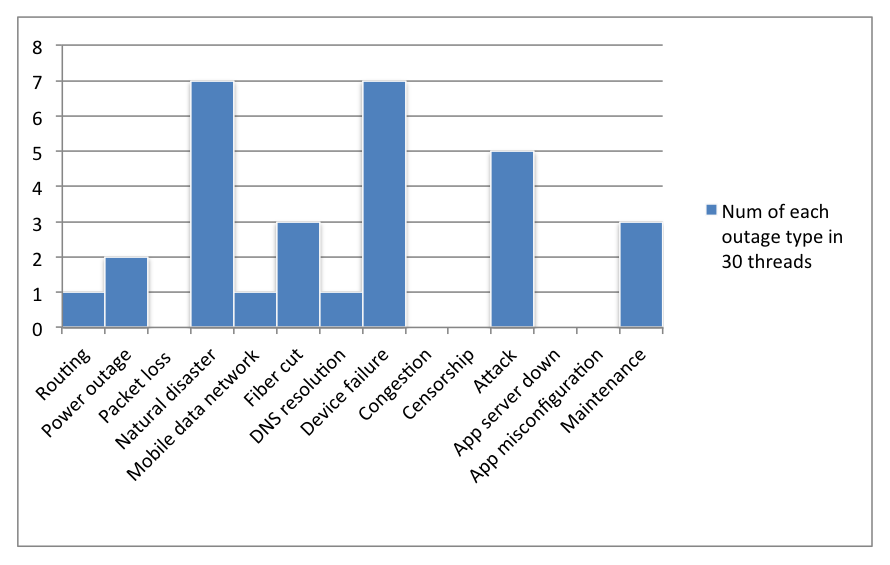
\epsfig{file=3.eps, height=1.5in, width=3in}
\caption{Num of Outage type in the 30 threads}
\end{figure}

\subsection{Choice of algorithm}
Because the outage type is discrete, so we can use classification method to solve the problem. But due to the types is multiple(14 types), so if we use multi-classification method, the difficulty will increased largely  and time efficiency is very low. So we decide to use multiple binary classifiers to avoid the multi-classification. Instead of partitioning the dataset into N categories, we learn a “concept” for each category independently; i.e., a binary classifier trying to determine whether a thread belongs in a particular category or not. So based on this method, we should classify the dataset 14 times to get all type of outage classification. Compared to classify the dataset one time using multi-classification, this method largely decreases the difficulty and largely improve the efficiency. For solving the binary classification problem, we think the best solution is Support Vector Machine(SVM). SVMs are supervised learning models with associated learning algorithms that analyze data and recognize patterns, used for classification and regression analysis. Given a set of training examples, each marked as belonging to one of two categories, an SVM training algorithm builds a model that assigns new examples into one category or the other, making it a non-probabilistic binary linear classifier. It has some advantages than other machine learning methods:
\begin{enumerate}
\item{it has a regularisation parameter, which makes the user think about avoiding over-fitting}
\item{it maximizes margin, so the model is slightly more robust}
\item{it uses the kernel trick, so you can build in expert knowledge about the problem via engineering the kernel}
\end{enumerate}
Besides, we will also evaluate the goodness of the learning step using a standard 10-fold cross-validation into the SVM algorithm. In 10-fold cross-validation, the original sample is randomly partitioned into 10 equal size subsamples. Of the 10 subsamples, a single subsample is retained as the validation data for testing the model, and the remaining 9 subsamples are used as training data. The cross-validation process is then repeated 10 times, with each of the 10 subsamples used exactly once as the validation data. The 10 results from the folds can then be averaged (or otherwise combined) to produce a single estimation. The advantage of this method over repeated random sub-sampling is that all observations are used for both training and validation, and each observation is used for validation exactly once.

\section{Implementation and Preliminary Result}
For the implementation, we decide to user a linear-kernel SVM for classification using the LibSVM toolkit which performed well in terms of both accuracy and speed. LibSVM toolkit is an integrated software for support vector classification, regression and distribution estimation. It also supports multi-class classification. 
\par From now we use the toolkit into our first 30 data-preprocessed try data, we use the first 15 threads to train the classifier and use the next 15 threads to test the classifier’s performance that we trained. The table 2 shows the accuracy of the 14 outage types prediction and the average of our trained classifier is 92.857\%. From the table, we can see that the accuracy of the outage types prediction is extremely well(most of them are 100\%). We think there are some reasons for getting this extremely well result:
\par The number of training data is not enough. We know that if we do the classification, we must have a large number of training data to train the classifier. But our first try-data is not enough, it will result in the classifier is not general to all the possible situations.
\par The number of predicted data is not enough. The predicted data may be just match this trained classifier well, it not represent the general situations.
\par In the data-preprocess step, we remove many unrelated content of the text, so the noise of the data is very small. It may result in a better result for classification.
In the future, we will improve the first two factors.

\begin{table}[h]
\centering
\begin{tabular}{ | l || c | }
  \hline
  Outage types & classification accuracy \\
  \hline
  Routing & 93.3333\% \\
  \hline
  Power outage & 100\%  \\
  \hline
  Packet loss & 100\%  \\
  \hline
  Natural disaster & 66.6667\%  \\
  \hline
  Mobile data network & 100\%  \\
  \hline
  Fiber cut & 80\%  \\
  \hline
  DNS resolution & 100\%  \\
  \hline
  Device failure & 60\%  \\
  \hline
  Congestion & 100\%  \\
  \hline
  Censorship & 100\%   \\
  \hline
  Attack & 100\%   \\
  \hline
  Application server & 100\%   \\
  \hline
  Application configuration & 100\%   \\
  \hline
  Maintenance & 100\%   \\
  \hline
  Average accuracy & 92.85714286\%   \\
  \hline
\end{tabular}
\caption{Classification result}\label{table:classification}
\end{table}

\section{Future Plans}
\paragraph{Beside the tasks that we implemented so far, there are more things that we can do in order to improve the accuracy and efficiency of this project, such as use linear-kernel SVM, enlarge the size of test data and test our classifier with new data}

\subsection{Data Enlarge}
Because we just use small samples to try our method for the runtime consideration, we will enlarge our data using in the method.
\subsection{Get a reasonable result for the outage type classification prediction}
Get a reasonable classifier that predict a new thread which belongs to what outage type. The result can basically match the thread’s actual  outage type.

\section{What we have done}
In this paper, we have integrated the posts with the same subject to the same thread in the mailing list. Furthermore, we have extracted and omitted the unessential data information and maintain the important data information for our classifier by using a stop words list that was obtained from the SMART information retrieval system[5]. We manually increased the amount of words in the stop words list from 571 to 1514, labeled thirty threads as our training data and used python Natural Language Toolkit(NLTK) to lemmatiz the data and improve the classification. Then, we tried out TF-IDF and found out that a word with high td-idf value within a thread doesn't mean the word is useful for the classification; as the result, we imported name-word library and city-word library of python Natural Language Toolkit(NLTK) to avoid this situation. After this, we generated two-dimensional matrix and obtained the useful data for our classification and got the classification result.

\begin{thebibliography}{7}
\bibitem{Kristen}
Kristen Carosa (2014, Dec 11),
  \emph{Widespread FairPoint Internet outage affects NH customers}. Retrieved from http://www.wmur.com/money/widespread-fairpoint-internet-outage-affecting-nh-customers/30176172

\bibitem{Mary}
Mary Scott (2014, September 5),
  \emph{Pellissippi State internet outage impacts all 5 campuses}.
Retrieved from http://www.wbir.com/story/news/local
\newline /2014/09/05/pellissippi-state-internet-outage-impacts-all-5-campuses/15152481/
  
\bibitem{Ritwik}
Ritwik Banerjee, Abbas Razaghpanah, Luis Chiang, Akassh Mishra, Vyas Sekar, Yejin Choi, Phillipa Gill,
  \emph{Internet Outages, the Eyewitness Accounts: Analysis of the Outages Mailing List}, 2013
  
\bibitem{Rode}
V.Rode.
\emph{Outages–outages(planned &unplanned) reporting}. 
Retrieved from https://puck.nether. net/mailman/listinfo/outages

\bibitem{Rocchio}
  J. J. Rocchio.
  \emph{Relevance feedback in information retrieval},1971. Retrieved from http://jmlr.org/papers/volume5/lewis04a/a11-smart-stop-list/english.stop

\bibitem{Ramos}
  J. Ramos.
  \emph{Using TF-IDF to determine word relevance in document queries} In Proc. Inter- national Conference on Machine Learning (ICML), 2003.
  
\bibitem{outages.org}
  virendra.rode@outages.org
  \emph{Internet outages mailing list}, 2006. Retrieved from
https://puck.nether.net/mailman/listinfo/outages

\end{thebibliography}
\end{document}